% Created by tikzDevice version 0.6.0 on 2011-04-12 19:43:47
% !TEX encoding = UTF-8 Unicode
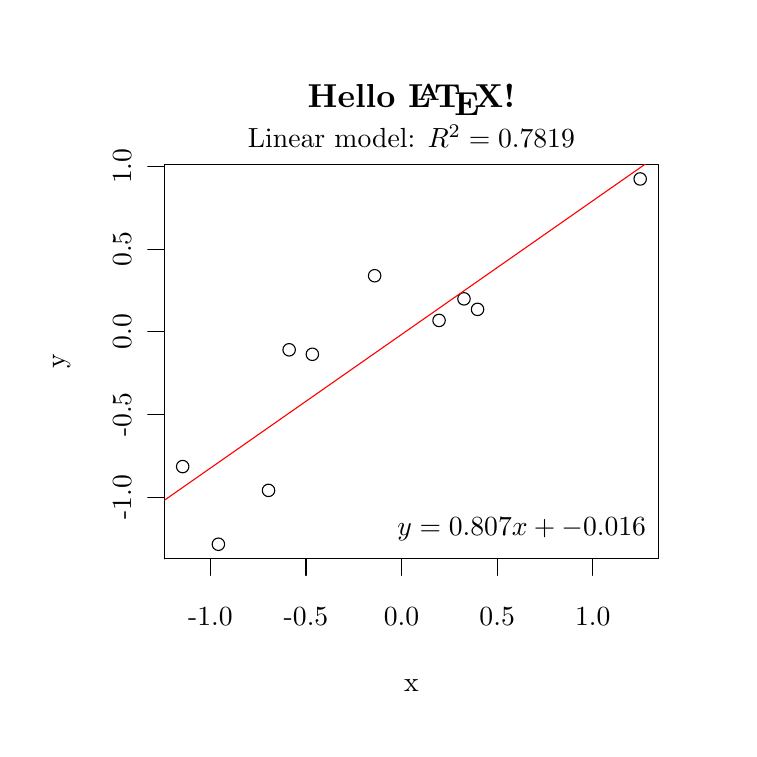
\begin{tikzpicture}[x=1pt,y=1pt]
\draw[color=white,opacity=0] (0,0) rectangle (252.94,252.94);
\begin{scope}
\path[clip] ( 49.20, 61.20) rectangle (227.75,203.75);
\definecolor[named]{drawColor}{rgb}{0.00,0.00,0.00}

\draw[color=drawColor,line cap=round,line join=round,fill opacity=0.00,] (157.46,155.15) circle (  2.25);

\draw[color=drawColor,line cap=round,line join=round,fill opacity=0.00,] ( 68.72, 66.48) circle (  2.25);

\draw[color=drawColor,line cap=round,line join=round,fill opacity=0.00,] (102.67,135.12) circle (  2.25);

\draw[color=drawColor,line cap=round,line join=round,fill opacity=0.00,] (125.18,163.50) circle (  2.25);

\draw[color=drawColor,line cap=round,line join=round,fill opacity=0.00,] ( 86.83, 85.94) circle (  2.25);

\draw[color=drawColor,line cap=round,line join=round,fill opacity=0.00,] (148.45,147.35) circle (  2.25);

\draw[color=drawColor,line cap=round,line join=round,fill opacity=0.00,] (221.13,198.47) circle (  2.25);

\draw[color=drawColor,line cap=round,line join=round,fill opacity=0.00,] ( 55.81, 94.54) circle (  2.25);

\draw[color=drawColor,line cap=round,line join=round,fill opacity=0.00,] ( 94.28,136.74) circle (  2.25);

\draw[color=drawColor,line cap=round,line join=round,fill opacity=0.00,] (162.36,151.35) circle (  2.25);
\end{scope}
\begin{scope}
\path[clip] (  0.00,  0.00) rectangle (252.94,252.94);
\definecolor[named]{drawColor}{rgb}{0.00,0.00,0.00}

\draw[color=drawColor,line cap=round,line join=round,fill opacity=0.00,] ( 65.83, 61.20) -- (203.98, 61.20);

\draw[color=drawColor,line cap=round,line join=round,fill opacity=0.00,] ( 65.83, 61.20) -- ( 65.83, 55.20);

\draw[color=drawColor,line cap=round,line join=round,fill opacity=0.00,] (100.37, 61.20) -- (100.37, 55.20);

\draw[color=drawColor,line cap=round,line join=round,fill opacity=0.00,] (134.91, 61.20) -- (134.91, 55.20);

\draw[color=drawColor,line cap=round,line join=round,fill opacity=0.00,] (169.45, 61.20) -- (169.45, 55.20);

\draw[color=drawColor,line cap=round,line join=round,fill opacity=0.00,] (203.98, 61.20) -- (203.98, 55.20);

\node[color=drawColor,anchor=base,inner sep=0pt, outer sep=0pt, scale=  1.00] at ( 65.83, 37.20) {-1.0%
};

\node[color=drawColor,anchor=base,inner sep=0pt, outer sep=0pt, scale=  1.00] at (100.37, 37.20) {-0.5%
};

\node[color=drawColor,anchor=base,inner sep=0pt, outer sep=0pt, scale=  1.00] at (134.91, 37.20) {0.0%
};

\node[color=drawColor,anchor=base,inner sep=0pt, outer sep=0pt, scale=  1.00] at (169.45, 37.20) {0.5%
};

\node[color=drawColor,anchor=base,inner sep=0pt, outer sep=0pt, scale=  1.00] at (203.98, 37.20) {1.0%
};

\draw[color=drawColor,line cap=round,line join=round,fill opacity=0.00,] ( 49.20, 83.41) -- ( 49.20,203.05);

\draw[color=drawColor,line cap=round,line join=round,fill opacity=0.00,] ( 49.20, 83.41) -- ( 43.20, 83.41);

\draw[color=drawColor,line cap=round,line join=round,fill opacity=0.00,] ( 49.20,113.32) -- ( 43.20,113.32);

\draw[color=drawColor,line cap=round,line join=round,fill opacity=0.00,] ( 49.20,143.23) -- ( 43.20,143.23);

\draw[color=drawColor,line cap=round,line join=round,fill opacity=0.00,] ( 49.20,173.14) -- ( 43.20,173.14);

\draw[color=drawColor,line cap=round,line join=round,fill opacity=0.00,] ( 49.20,203.05) -- ( 43.20,203.05);

\node[rotate= 90.00,color=drawColor,anchor=base,inner sep=0pt, outer sep=0pt, scale=  1.00] at ( 37.20, 83.41) {-1.0%
};

\node[rotate= 90.00,color=drawColor,anchor=base,inner sep=0pt, outer sep=0pt, scale=  1.00] at ( 37.20,113.32) {-0.5%
};

\node[rotate= 90.00,color=drawColor,anchor=base,inner sep=0pt, outer sep=0pt, scale=  1.00] at ( 37.20,143.23) {0.0%
};

\node[rotate= 90.00,color=drawColor,anchor=base,inner sep=0pt, outer sep=0pt, scale=  1.00] at ( 37.20,173.14) {0.5%
};

\node[rotate= 90.00,color=drawColor,anchor=base,inner sep=0pt, outer sep=0pt, scale=  1.00] at ( 37.20,203.05) {1.0%
};

\draw[color=drawColor,line cap=round,line join=round,fill opacity=0.00,] ( 49.20, 61.20) --
	(227.75, 61.20) --
	(227.75,203.75) --
	( 49.20,203.75) --
	( 49.20, 61.20);
\end{scope}
\begin{scope}
\path[clip] (  0.00,  0.00) rectangle (252.94,252.94);
\definecolor[named]{drawColor}{rgb}{0.00,0.00,0.00}

\node[color=drawColor,anchor=base,inner sep=0pt, outer sep=0pt, scale=  1.20] at (138.47,224.20) {\bfseries Hello \LaTeX!%
};

\node[color=drawColor,anchor=base,inner sep=0pt, outer sep=0pt, scale=  1.00] at (138.47, 13.20) {x%
};

\node[rotate= 90.00,color=drawColor,anchor=base,inner sep=0pt, outer sep=0pt, scale=  1.00] at ( 13.20,132.47) {y%
};
\end{scope}
\begin{scope}
\path[clip] ( 49.20, 61.20) rectangle (227.75,203.75);
\definecolor[named]{drawColor}{rgb}{1.00,0.00,0.00}

\draw[color=drawColor,line cap=round,line join=round,fill opacity=0.00,] ( 49.20, 82.37) -- (227.74,207.18);
\end{scope}
\begin{scope}
\path[clip] (  0.00,  0.00) rectangle (252.94,252.94);
\definecolor[named]{drawColor}{rgb}{0.00,0.00,0.00}

\node[color=drawColor,anchor=base,inner sep=0pt, outer sep=0pt, scale=  1.00] at (138.47,209.75) {Linear model: $R^{2}= 0.7819 $%
};
\end{scope}
\begin{scope}
\path[clip] ( 49.20, 61.20) rectangle (227.75,203.75);
\definecolor[named]{drawColor}{rgb}{0.00,0.00,0.00}

\node[color=drawColor,anchor=base west,inner sep=0pt, outer sep=0pt, scale=  1.00] at (133.38, 69.76) {$y = 0.807x +-0.016$%
};
\end{scope}
\end{tikzpicture}
